\chapter{Instrumentation for real-time operation 
{\color{magenta}{Contributing author: COM, ES, JB}}}
%\\ \color{green} POST PUBLIC REVIEW VERSION\color{black}} 
    \label{ch:instrumentation}

\noindent
\begin{tcolorbox}
\parbox{\textwidth}{
\emph{\textbf{Key Points}\\
In this section currently applied as well as instrumentation that is under development is being described... 
}}
\end{tcolorbox}



The following is a list of available instrumentation that will be discussed in detail in this chapter and recommendations made in how to setup these instruments and which implications the use of the various instruments have on data quality and usability in the operational real-time context in the energy industry.

Typical instrumentation for meteorological measurements in wind power context are divided into two categories: 
\begin{itemize}
    \item meteorological masts
        \begin{itemize}
            \item cup anemometers
            \item sonic anemometers
             \item temperature sensors
             \item pressure sensors
             \item hygrometer sensors
             \item precipitation sensors rain gauges   
        \end{itemize}
    \item remote sensing instruments
        \begin{itemize}
            \item Wind Profiling Radar
            \item SODAR
            \item LiDAR 	
                \begin{itemize}
                    \item Wind Profiling LiDAR
                    \item Scanning LiDAR (Long-Range and short-range wind tracer)
                \end{itemize}
        \end{itemize}
\end{itemize}


Not so common instrumentation or additional instrumentation are:
\begin{itemize}
    \item Microwave Radiometers (measures energy emitted at sub-millimetre-to-centimetre wavelengths at frequencies of 1–1000GHz)  
    \item Ceilometer (light source to determine the height of a cloud base. Ceilometers can also be used to measure the aerosol)
    \item Microbarographs (measures atmospheric pressure)
\end{itemize}

These instrumentation are more commonly used in research measurement campaigns and in meteorological projects. Literature on these types such as microwave radiometers are described by e.g.  \cite{Ulaby1982,Matzler2006}, for ceilometers by \cite{Morris2016}, or microbarographs by \cite{Monserrat1992}.



Typical instrumentation for meteorological measurement campaigns in the solar power context are divided into two categories: 
\begin{itemize}
    \item Solar Radiation Sensors
        \begin{itemize}
            \item Pyranometers 
            \item Pyrheliometer
            \item Rotating Shadowband Irradiometer
            \item Sun Tracker
            \item Reference Cell (e.g. Silikon Irradiance sensor)
            \item Sunshine Duration Sensor
        \end{itemize}
    \item Met Stations
        \begin{itemize}
            \item cup anemometers
            \item sonic anemometers
             \item temperature sensors
             \item pressure sensors
             \item hygrometer sensors
             \item precipitation sensors rain gauges   
        \end{itemize}
\end{itemize}




\section{Meteorological masts} \label{subsec:meteorological_masts}

Meteorological mast are still the most commonly used measurement instrumentation for the planning phase and operation of wind farms. An example is shown in Figure 2. 


\begin{figure}[h!]
\center
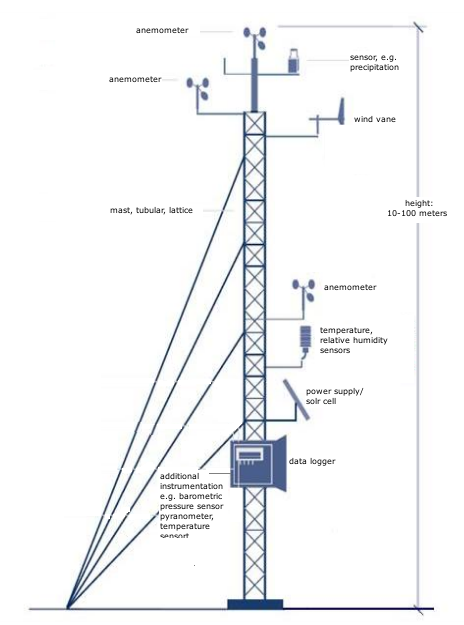
\includegraphics[width=0.5\textwidth]{figures/typical_met_mast.png}
\caption{Example of a typical met mast with various instrumentation, data logger, power supply and wiring. Typical instrumentation are cup anemometers or sonic anemometers, wind vanes, temperature, pressure and air density sensors, pyranometers and precipitation and humidity  sensors.}
\label{fig:met_mast}
\end{figure}






\section{Remote Sensing Instrumentation {\color{magenta}{Contributing author: ES}}}\label{sec:remote-sensing}




\section{Solar Radiation Sensors }\label{sec:solarradiation}


\section{Instrumentation on Met stations }\label{sec:metstations}


\section{SCADA Power Measurement Systems {\color{magenta}{Contributing author: JB}}}\label{sec:scadasystems}

\subsection{Wind Power SCADA systems }\label{subsec:scadasolar}

Suggested content:
\begin{itemize}
    \item Turbine anemometer (and issues)
    \item Relevant turbine SCADA parameters
    \item Relevant derived quantities (e.g. rotor effective wind speed, power available)
    \item ???
\end{itemize}

\subsection{Solar Power SCADA Systems }\label{subsec:scadawind}


%\section{}\label{sec:}

%\subsection{}\label{subsec:}
